Il mio proggeto di tesi ha l'ambizione di creare una piattaforma che consenta a utenti e aziende di creare la propria piattaforma di E-Learning.
La scelta del progetto è stata dettata dal crescente interesse nei confronti di tali piattaforme  negli ultimi anni.
Oggi giorno è facile confondere sistemi di e-learning con i MOOC (Massive Open Online Course), la differenza sostanzizale sta nel fatto che quest'ultimi sono corsi aperti a chiunque,la partecipazione è gratuita e permettono interattività tra gli studenti.
Il primo MOOC nasce intorno al 2007, grazie al lavoro del Professor O’Donnell, dell'Università della Pennsylvania.
L'enorme potenziale di queste piattaforme è stata compresa sin da subito e ha portato alla nascita di diversi piattaforme come Coursera, EdX, Udacity.
La Maggior parte di queste piattaforme offrono corsi organizzati direttamente dagli atenei tra cui troviamo nomi prestigiosi come Stanford, Harvard, Berkeley, MIT. In generale i corsi ricoprono diverse tematiche e vengono erogati direttamente dai Professori degli atenei universitari.
Tutti i corsi sono gratuiti cavalcando la filosofia tipica dei MOOC, viene pero richiesto un compenso nel caso in cui si desidera ottenere una certificazione, rilasciata solo dopo aver superato test per verificcare il livello di apprendimento.

\begin{figure}[htb] %  figure placement: here, top, bottom
 \centering
 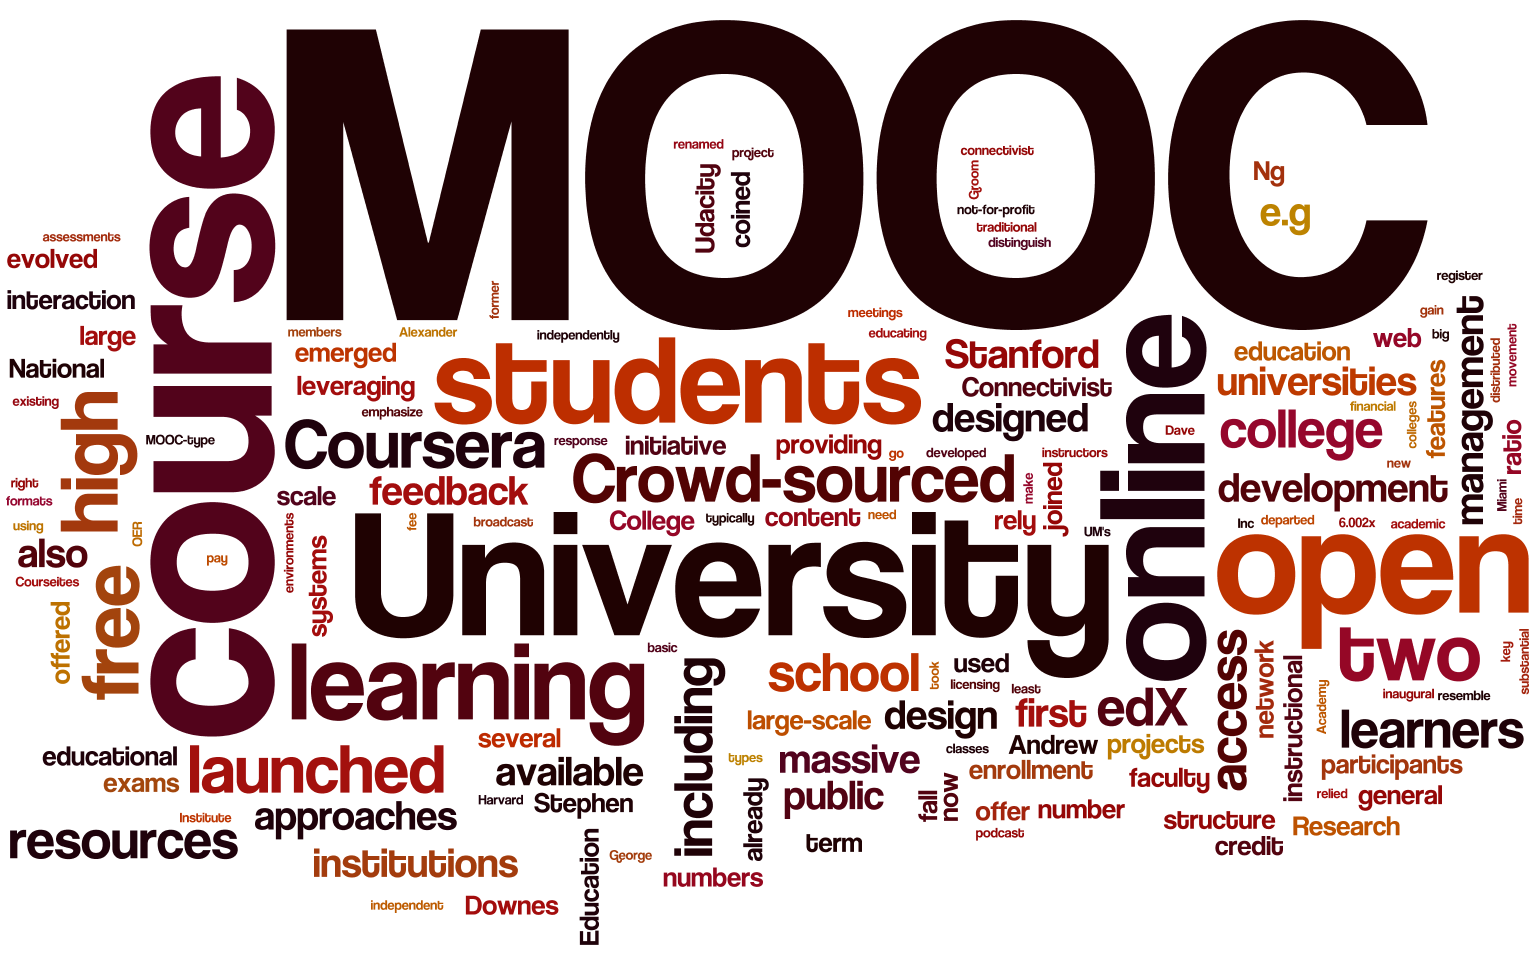
\includegraphics[width=0.8\linewidth]{images/introduction/mooc.png}\hfill
 \caption[Mooc image]{Mooc image}
 \label{fig:fourV}
\end{figure}

Questi sistemi sono stati accolti come una vera e propria rivoluzione nel mondo dell'istruzione, rendono la formazione accessibile a chiunque eliminando barriere temporali e spaziali. Infatti la comodità e il vantggio di queste piattaforme è poter seguire corsi di università a migliaia di chilometri di distanza comodamente da casa e in qualsiasi momento e orario della giornata.

Nelle prime piattaforme di MOOC i corsi erano quindi tenuti dagli stessi docenti degli atenei, questo trend è pero cambiato negli ultimi anni e ha visto la nascita di piattaforme in cui chiunque può creare un proprio corso.

Questa nuova opportunità che viene offerta per esempio dalla piattaforma Udemy, ha riscontrato subito un grande successo ed è stata sfruttata da molte persone che ne hanno fatto una vera e propria fonte di guadagno. 

Il mio progetto è invece indirizzato a tutti gli utenti privati, aziende, scuole che vogliono creare una propria piattaforma dove vengono offerti esclusivamente i loro corsi.

Creare un serizio di e-learning richiede investimenti importanti per coprire i costi di realizzazione, storage e traffico dati per lo streaming  dei contenuti video.

Già di per se tali costi potrebbero scoragiare un utente medio, inoltre la realizzazione richiede conoscenze tecniche, per la gestione dei video ma anche per lo streaming.
Infatti nonostante HTML5 la gestione dei video è molto insidiosa, non esiste un standard per lo streaming e inoltre bisogna garantire la fruzione dei contenuti su diversi dispositivi.
Quest'ultimo ostacolo potrebbe essere risolto tramite l'utilizzo di HLS(HTTP Live Streaming) protocollo di comunicazione concepito da Apple e basato su HTTP, che separa il flusso video in chunk e adatta la qualità video sulla base del dispositivo e della connessione.

Infine un ultimo ostacolo potrebbe essere rappresentato 

